\documentclass[twoside]{book}

% Packages required by doxygen
\usepackage{calc}
\usepackage{doxygen}
\usepackage{graphicx}
\usepackage[utf8]{inputenc}
\usepackage{makeidx}
\usepackage{multicol}
\usepackage{multirow}
\usepackage{textcomp}
\usepackage[table]{xcolor}

% Font selection
\usepackage[T1]{fontenc}
\usepackage{mathptmx}
\usepackage[scaled=.90]{helvet}
\usepackage{courier}
\usepackage{amssymb}
\usepackage{sectsty}
\renewcommand{\familydefault}{\sfdefault}
\allsectionsfont{%
  \fontseries{bc}\selectfont%
  \color{darkgray}%
}
\renewcommand{\DoxyLabelFont}{%
  \fontseries{bc}\selectfont%
  \color{darkgray}%
}

% Page & text layout
\usepackage{geometry}
\geometry{%
  a4paper,%
  top=2.5cm,%
  bottom=2.5cm,%
  left=2.5cm,%
  right=2.5cm%
}
\tolerance=750
\hfuzz=15pt
\hbadness=750
\setlength{\emergencystretch}{15pt}
\setlength{\parindent}{0cm}
\setlength{\parskip}{0.2cm}
\makeatletter
\renewcommand{\paragraph}{%
  \@startsection{paragraph}{4}{0ex}{-1.0ex}{1.0ex}{%
    \normalfont\normalsize\bfseries\SS@parafont%
  }%
}
\renewcommand{\subparagraph}{%
  \@startsection{subparagraph}{5}{0ex}{-1.0ex}{1.0ex}{%
    \normalfont\normalsize\bfseries\SS@subparafont%
  }%
}
\makeatother

% Headers & footers
\usepackage{fancyhdr}
\pagestyle{fancyplain}
\fancyhead[LE]{\fancyplain{}{\bfseries\thepage}}
\fancyhead[CE]{\fancyplain{}{}}
\fancyhead[RE]{\fancyplain{}{\bfseries\leftmark}}
\fancyhead[LO]{\fancyplain{}{\bfseries\rightmark}}
\fancyhead[CO]{\fancyplain{}{}}
\fancyhead[RO]{\fancyplain{}{\bfseries\thepage}}
\fancyfoot[LE]{\fancyplain{}{}}
\fancyfoot[CE]{\fancyplain{}{}}
\fancyfoot[RE]{\fancyplain{}{\bfseries\scriptsize Generated on Tue Mar 18 2014 11\-:32\-:42 for Tornado\-Server\-M\-I by Doxygen }}
\fancyfoot[LO]{\fancyplain{}{\bfseries\scriptsize Generated on Tue Mar 18 2014 11\-:32\-:42 for Tornado\-Server\-M\-I by Doxygen }}
\fancyfoot[CO]{\fancyplain{}{}}
\fancyfoot[RO]{\fancyplain{}{}}
\renewcommand{\footrulewidth}{0.4pt}
\renewcommand{\chaptermark}[1]{%
  \markboth{#1}{}%
}
\renewcommand{\sectionmark}[1]{%
  \markright{\thesection\ #1}%
}

% Indices & bibliography
\usepackage{natbib}
\usepackage[titles]{tocloft}
\setcounter{tocdepth}{3}
\setcounter{secnumdepth}{5}
\makeindex

% Hyperlinks (required, but should be loaded last)
\usepackage{ifpdf}
\ifpdf
  \usepackage[pdftex,pagebackref=true]{hyperref}
\else
  \usepackage[ps2pdf,pagebackref=true]{hyperref}
\fi
\hypersetup{%
  colorlinks=true,%
  linkcolor=blue,%
  citecolor=blue,%
  unicode%
}

% Custom commands
\newcommand{\clearemptydoublepage}{%
  \newpage{\pagestyle{empty}\cleardoublepage}%
}


%===== C O N T E N T S =====

\begin{document}

% Titlepage & ToC
\hypersetup{pageanchor=false}
\pagenumbering{roman}
\begin{titlepage}
\vspace*{7cm}
\begin{center}%
{\Large Tornado\-Server\-M\-I \\[1ex]\large 0.\-3 }\\
\vspace*{1cm}
{\large Generated by Doxygen 1.8.6}\\
\vspace*{0.5cm}
{\small Tue Mar 18 2014 11:32:42}\\
\end{center}
\end{titlepage}
\clearemptydoublepage
\tableofcontents
\clearemptydoublepage
\pagenumbering{arabic}
\hypersetup{pageanchor=true}

%--- Begin generated contents ---
\chapter{ptut}
\label{md__r_e_a_d_m_e}
\hypertarget{md__r_e_a_d_m_e}{}
ptut 
\chapter{Namespace Index}
\section{Packages}
Here are the packages with brief descriptions (if available)\-:\begin{DoxyCompactList}
\item\contentsline{section}{\hyperlink{namespacesuper_tornado}{super\-Tornado} }{\pageref{namespacesuper_tornado}}{}
\end{DoxyCompactList}

\chapter{Hierarchical Index}
\section{Class Hierarchy}
This inheritance list is sorted roughly, but not completely, alphabetically\-:\begin{DoxyCompactList}
\item \contentsline{section}{m.\-log.\-bcolors}{\pageref{classm_1_1log_1_1bcolors}}{}
\item Exception\begin{DoxyCompactList}
\item \contentsline{section}{m.\-load\-Conf.\-Config\-Error}{\pageref{classm_1_1load_conf_1_1_config_error}}{}
\end{DoxyCompactList}
\item Filter\begin{DoxyCompactList}
\item \contentsline{section}{m.\-log.\-Single\-Level\-Filter}{\pageref{classm_1_1log_1_1_single_level_filter}}{}
\end{DoxyCompactList}
\item \contentsline{section}{super\-Tornado.\-Global\-Vars}{\pageref{classsuper_tornado_1_1_global_vars}}{}
\item \contentsline{section}{m.\-log.\-lvl}{\pageref{classm_1_1log_1_1lvl}}{}
\item object\begin{DoxyCompactList}
\item \contentsline{section}{m.\-load\-Conf.\-Load\-Conf}{\pageref{classm_1_1load_conf_1_1_load_conf}}{}
\item \contentsline{section}{m.\-log.\-Log}{\pageref{classm_1_1log_1_1_log}}{}
\item \contentsline{section}{m.\-login.\-Login}{\pageref{classm_1_1login_1_1_login}}{}
\end{DoxyCompactList}
\item Request\-Handler\begin{DoxyCompactList}
\item \contentsline{section}{super\-Tornado.\-Base\-Handler}{\pageref{classsuper_tornado_1_1_base_handler}}{}
\begin{DoxyCompactList}
\item \contentsline{section}{super\-Tornado.\-Disconnection\-Handler}{\pageref{classsuper_tornado_1_1_disconnection_handler}}{}
\item \contentsline{section}{super\-Tornado.\-Main\-Handler}{\pageref{classsuper_tornado_1_1_main_handler}}{}
\item \contentsline{section}{super\-Tornado.\-Unauthorized\-Handler}{\pageref{classsuper_tornado_1_1_unauthorized_handler}}{}
\item \contentsline{section}{super\-Tornado.\-Video\-Handler}{\pageref{classsuper_tornado_1_1_video_handler}}{}
\item \contentsline{section}{super\-Tornado.\-W\-Socket\-Handler}{\pageref{classsuper_tornado_1_1_w_socket_handler}}{}
\end{DoxyCompactList}
\end{DoxyCompactList}
\item Web\-Socket\-Handler\begin{DoxyCompactList}
\item \contentsline{section}{super\-Tornado.\-W\-Socket\-Handler}{\pageref{classsuper_tornado_1_1_w_socket_handler}}{}
\end{DoxyCompactList}
\end{DoxyCompactList}

\chapter{Class Index}
\section{Class List}
Here are the classes, structs, unions and interfaces with brief descriptions\-:\begin{DoxyCompactList}
\item\contentsline{section}{\hyperlink{classsuper_tornado_1_1_base_handler}{super\-Tornado.\-Base\-Handler} }{\pageref{classsuper_tornado_1_1_base_handler}}{}
\item\contentsline{section}{\hyperlink{classm_1_1log_1_1bcolors}{m.\-log.\-bcolors} }{\pageref{classm_1_1log_1_1bcolors}}{}
\item\contentsline{section}{\hyperlink{classm_1_1load_conf_1_1_config_error}{m.\-load\-Conf.\-Config\-Error} }{\pageref{classm_1_1load_conf_1_1_config_error}}{}
\item\contentsline{section}{\hyperlink{classsuper_tornado_1_1_disconnection_handler}{super\-Tornado.\-Disconnection\-Handler} }{\pageref{classsuper_tornado_1_1_disconnection_handler}}{}
\item\contentsline{section}{\hyperlink{classsuper_tornado_1_1_global_vars}{super\-Tornado.\-Global\-Vars} }{\pageref{classsuper_tornado_1_1_global_vars}}{}
\item\contentsline{section}{\hyperlink{classm_1_1load_conf_1_1_load_conf}{m.\-load\-Conf.\-Load\-Conf} }{\pageref{classm_1_1load_conf_1_1_load_conf}}{}
\item\contentsline{section}{\hyperlink{classm_1_1log_1_1_log}{m.\-log.\-Log} }{\pageref{classm_1_1log_1_1_log}}{}
\item\contentsline{section}{\hyperlink{classm_1_1login_1_1_login}{m.\-login.\-Login} }{\pageref{classm_1_1login_1_1_login}}{}
\item\contentsline{section}{\hyperlink{classm_1_1log_1_1lvl}{m.\-log.\-lvl} }{\pageref{classm_1_1log_1_1lvl}}{}
\item\contentsline{section}{\hyperlink{classsuper_tornado_1_1_main_handler}{super\-Tornado.\-Main\-Handler} }{\pageref{classsuper_tornado_1_1_main_handler}}{}
\item\contentsline{section}{\hyperlink{classm_1_1log_1_1_single_level_filter}{m.\-log.\-Single\-Level\-Filter} }{\pageref{classm_1_1log_1_1_single_level_filter}}{}
\item\contentsline{section}{\hyperlink{classsuper_tornado_1_1_unauthorized_handler}{super\-Tornado.\-Unauthorized\-Handler} }{\pageref{classsuper_tornado_1_1_unauthorized_handler}}{}
\item\contentsline{section}{\hyperlink{classsuper_tornado_1_1_video_handler}{super\-Tornado.\-Video\-Handler} }{\pageref{classsuper_tornado_1_1_video_handler}}{}
\item\contentsline{section}{\hyperlink{classsuper_tornado_1_1_w_socket_handler}{super\-Tornado.\-W\-Socket\-Handler} }{\pageref{classsuper_tornado_1_1_w_socket_handler}}{}
\end{DoxyCompactList}

\chapter{Namespace Documentation}
\hypertarget{namespacesuper_tornado}{\section{super\-Tornado Namespace Reference}
\label{namespacesuper_tornado}\index{super\-Tornado@{super\-Tornado}}
}
\subsection*{Classes}
\begin{DoxyCompactItemize}
\item 
class \hyperlink{classsuper_tornado_1_1_global_vars}{Global\-Vars}
\item 
class \hyperlink{classsuper_tornado_1_1_base_handler}{Base\-Handler}
\item 
class \hyperlink{classsuper_tornado_1_1_main_handler}{Main\-Handler}
\item 
class \hyperlink{classsuper_tornado_1_1_video_handler}{Video\-Handler}
\item 
class \hyperlink{classsuper_tornado_1_1_unauthorized_handler}{Unauthorized\-Handler}
\item 
class \hyperlink{classsuper_tornado_1_1_disconnection_handler}{Disconnection\-Handler}
\item 
class \hyperlink{classsuper_tornado_1_1_w_socket_handler}{W\-Socket\-Handler}
\end{DoxyCompactItemize}
\subsection*{Variables}
\begin{DoxyCompactItemize}
\item 
tuple {\bfseries application}
\item 
\hypertarget{namespacesuper_tornado_acc65a75d3941165f9c5e66f6af6bd32f}{tuple {\bfseries http\-\_\-server} = tornado.\-httpserver.\-H\-T\-T\-P\-Server(application)}\label{namespacesuper_tornado_acc65a75d3941165f9c5e66f6af6bd32f}

\end{DoxyCompactItemize}


\subsection{Detailed Description}
\begin{DoxyVerb}Import Tornado Server\end{DoxyVerb}
 

\subsection{Variable Documentation}
\hypertarget{namespacesuper_tornado_a8fda9ce7efd1de41c7487a207de2f71d}{\index{super\-Tornado@{super\-Tornado}!application@{application}}
\index{application@{application}!superTornado@{super\-Tornado}}
\subsubsection[{application}]{\setlength{\rightskip}{0pt plus 5cm}tuple super\-Tornado.\-application}}\label{namespacesuper_tornado_a8fda9ce7efd1de41c7487a207de2f71d}
{\bfseries Initial value\-:}
\begin{DoxyCode}
1 = tornado.web.Application([
2     (\textcolor{stringliteral}{r"/"}, MainHandler),
3     (\textcolor{stringliteral}{r"/video"}, VideoHandler),
4     (\textcolor{stringliteral}{r"/unauthorized"}, UnauthorizedHandler),
5     (\textcolor{stringliteral}{r"/disconnection"}, DisconnectionHandler),
6     (\textcolor{stringliteral}{r"/socket"}, WSocketHandler),
7     (\textcolor{stringliteral}{r"/(favicon.ico)"}, tornado.web.StaticFileHandler,\{\textcolor{stringliteral}{"path"}:\textcolor{stringliteral}{"./v/images"}\},),
8     (\textcolor{stringliteral}{r"/style/(.*)"}, tornado.web.StaticFileHandler,\{\textcolor{stringliteral}{"path"}:\textcolor{stringliteral}{"./v/style"}\},),
9     (\textcolor{stringliteral}{r"/images/(.*)"}, tornado.web.StaticFileHandler,\{\textcolor{stringliteral}{"path"}:\textcolor{stringliteral}{"./v/images"}\},),
10     (\textcolor{stringliteral}{r"/js/(.*)"}, tornado.web.StaticFileHandler,\{\textcolor{stringliteral}{"path"}:\textcolor{stringliteral}{"./v/js"}\},)],
11     cookie\_secret=\textcolor{stringliteral}{''}.join(random.choice(string.ascii\_uppercase + string.digits) \textcolor{keywordflow}{for} \_ \textcolor{keywordflow}{in} range(64)))
\end{DoxyCode}

\chapter{Class Documentation}
\hypertarget{classsuper_tornado_1_1_base_handler}{\section{super\-Tornado.\-Base\-Handler Class Reference}
\label{classsuper_tornado_1_1_base_handler}\index{super\-Tornado.\-Base\-Handler@{super\-Tornado.\-Base\-Handler}}
}
Inheritance diagram for super\-Tornado.\-Base\-Handler\-:\begin{figure}[H]
\begin{center}
\leavevmode
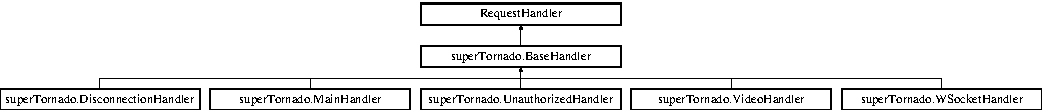
\includegraphics[height=1.473684cm]{classsuper_tornado_1_1_base_handler}
\end{center}
\end{figure}
\subsection*{Public Member Functions}
\begin{DoxyCompactItemize}
\item 
\hypertarget{classsuper_tornado_1_1_base_handler_aecb8cb2cc891c1012986d266958b981d}{def {\bfseries get\-\_\-current\-\_\-user}}\label{classsuper_tornado_1_1_base_handler_aecb8cb2cc891c1012986d266958b981d}

\end{DoxyCompactItemize}


\subsection{Detailed Description}
\begin{DoxyVerb}Define BaseHandler for create the basis for session connection
cookie secure  based (sign and timestamp )
\end{DoxyVerb}
 

The documentation for this class was generated from the following file\-:\begin{DoxyCompactItemize}
\item 
super\-Tornado.\-py\end{DoxyCompactItemize}

\hypertarget{classm_1_1log_1_1bcolors}{\section{m.\-log.\-bcolors Class Reference}
\label{classm_1_1log_1_1bcolors}\index{m.\-log.\-bcolors@{m.\-log.\-bcolors}}
}
\subsection*{Static Public Attributes}
\begin{DoxyCompactItemize}
\item 
\hypertarget{classm_1_1log_1_1bcolors_a930ec546f4b168584a472688b7f76159}{string {\bfseries D\-E\-B\-U\-G} = '\textbackslash{}033\mbox{[}94m'}\label{classm_1_1log_1_1bcolors_a930ec546f4b168584a472688b7f76159}

\item 
\hypertarget{classm_1_1log_1_1bcolors_ac1f6785cf1156a6e807bd34becae40cc}{string {\bfseries I\-N\-F\-O} = '\textbackslash{}033\mbox{[}95m'}\label{classm_1_1log_1_1bcolors_ac1f6785cf1156a6e807bd34becae40cc}

\item 
\hypertarget{classm_1_1log_1_1bcolors_a08e96f78e19ddcbeb35803253921a8d6}{string {\bfseries S\-U\-C\-C\-E\-S\-S} = '\textbackslash{}033\mbox{[}92m'}\label{classm_1_1log_1_1bcolors_a08e96f78e19ddcbeb35803253921a8d6}

\item 
\hypertarget{classm_1_1log_1_1bcolors_adf7b4f5d7944a6513fc8c41d6a5dc14b}{string {\bfseries W\-A\-R\-N\-I\-N\-G} = '\textbackslash{}033\mbox{[}93m'}\label{classm_1_1log_1_1bcolors_adf7b4f5d7944a6513fc8c41d6a5dc14b}

\item 
\hypertarget{classm_1_1log_1_1bcolors_aefe04c066409cd17944030d7c8f7da78}{string {\bfseries F\-A\-I\-L} = '\textbackslash{}033\mbox{[}91m'}\label{classm_1_1log_1_1bcolors_aefe04c066409cd17944030d7c8f7da78}

\item 
\hypertarget{classm_1_1log_1_1bcolors_a2ca52c51d05abcaa81c0c4703741cd0c}{string {\bfseries E\-N\-D\-C} = '\textbackslash{}033\mbox{[}0m'}\label{classm_1_1log_1_1bcolors_a2ca52c51d05abcaa81c0c4703741cd0c}

\end{DoxyCompactItemize}


\subsection{Detailed Description}
\begin{DoxyVerb}Define constant value color for different level
\end{DoxyVerb}
 

The documentation for this class was generated from the following file\-:\begin{DoxyCompactItemize}
\item 
m/log.\-py\end{DoxyCompactItemize}

\hypertarget{classm_1_1load_conf_1_1_config_error}{\section{m.\-load\-Conf.\-Config\-Error Class Reference}
\label{classm_1_1load_conf_1_1_config_error}\index{m.\-load\-Conf.\-Config\-Error@{m.\-load\-Conf.\-Config\-Error}}
}
Inheritance diagram for m.\-load\-Conf.\-Config\-Error\-:\begin{figure}[H]
\begin{center}
\leavevmode
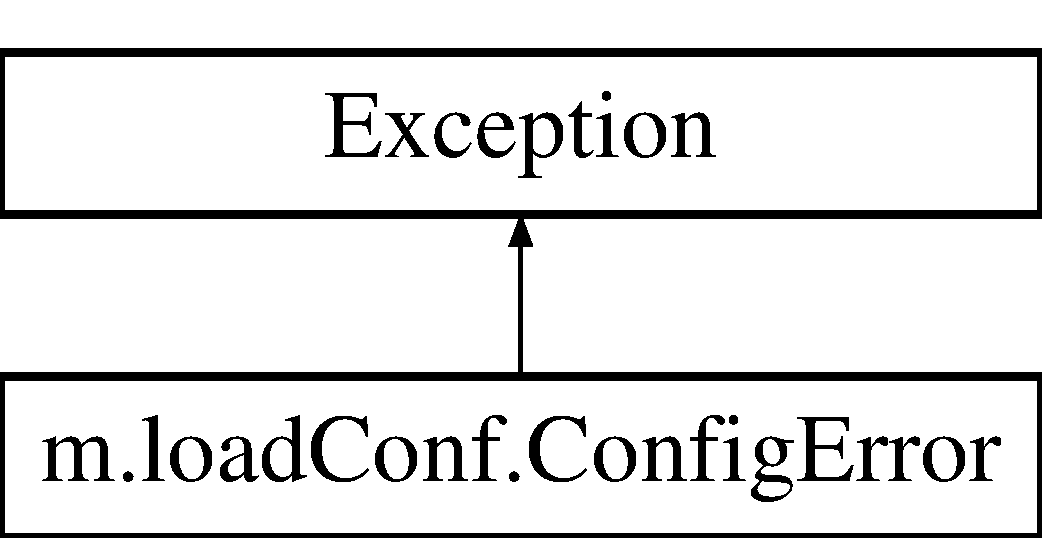
\includegraphics[height=2.000000cm]{classm_1_1load_conf_1_1_config_error}
\end{center}
\end{figure}
\subsection*{Public Member Functions}
\begin{DoxyCompactItemize}
\item 
\hypertarget{classm_1_1load_conf_1_1_config_error_a33facc9fac19952f7b5a88f7c8e32649}{def {\bfseries \-\_\-\-\_\-init\-\_\-\-\_\-}}\label{classm_1_1load_conf_1_1_config_error_a33facc9fac19952f7b5a88f7c8e32649}

\item 
\hypertarget{classm_1_1load_conf_1_1_config_error_a2da563460e4a813f567a8ff8e810036d}{def {\bfseries \-\_\-\-\_\-str\-\_\-\-\_\-}}\label{classm_1_1load_conf_1_1_config_error_a2da563460e4a813f567a8ff8e810036d}

\end{DoxyCompactItemize}
\subsection*{Public Attributes}
\begin{DoxyCompactItemize}
\item 
\hypertarget{classm_1_1load_conf_1_1_config_error_af6b99671bc89ab2fd2195aa8711c9380}{{\bfseries value}}\label{classm_1_1load_conf_1_1_config_error_af6b99671bc89ab2fd2195aa8711c9380}

\end{DoxyCompactItemize}


\subsection{Detailed Description}
\begin{DoxyVerb}Exception : error loading configuration\end{DoxyVerb}
 

The documentation for this class was generated from the following file\-:\begin{DoxyCompactItemize}
\item 
m/load\-Conf.\-py\end{DoxyCompactItemize}

\hypertarget{classsuper_tornado_1_1_disconnection_handler}{\section{super\-Tornado.\-Disconnection\-Handler Class Reference}
\label{classsuper_tornado_1_1_disconnection_handler}\index{super\-Tornado.\-Disconnection\-Handler@{super\-Tornado.\-Disconnection\-Handler}}
}
Inheritance diagram for super\-Tornado.\-Disconnection\-Handler\-:\begin{figure}[H]
\begin{center}
\leavevmode
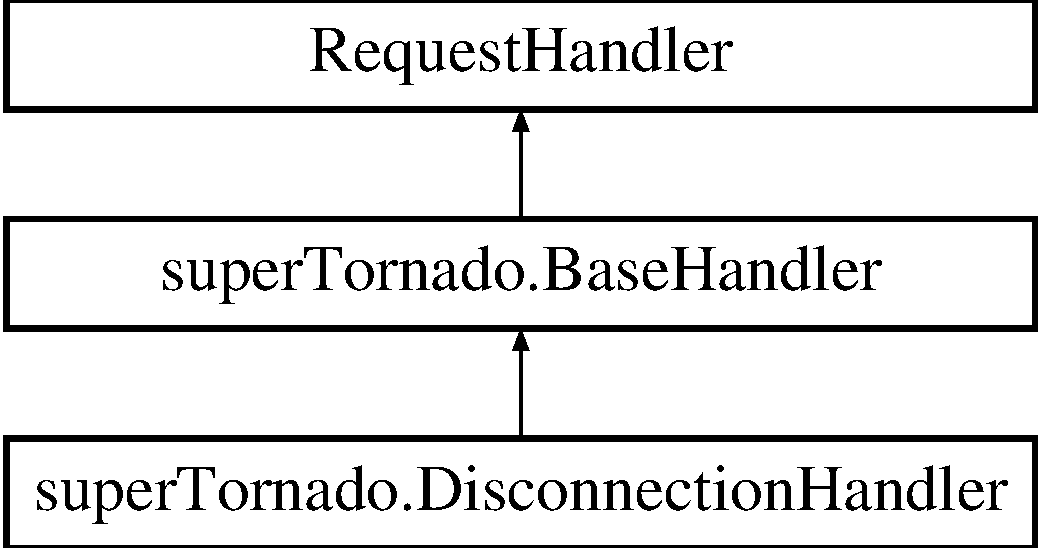
\includegraphics[height=3.000000cm]{classsuper_tornado_1_1_disconnection_handler}
\end{center}
\end{figure}
\subsection*{Public Member Functions}
\begin{DoxyCompactItemize}
\item 
def \hyperlink{classsuper_tornado_1_1_disconnection_handler_a342baf9e09790a755c5fd85f115c6198}{get}
\end{DoxyCompactItemize}


\subsection{Detailed Description}
\begin{DoxyVerb}/disconnection in http server
\end{DoxyVerb}
 

\subsection{Member Function Documentation}
\hypertarget{classsuper_tornado_1_1_disconnection_handler_a342baf9e09790a755c5fd85f115c6198}{\index{super\-Tornado\-::\-Disconnection\-Handler@{super\-Tornado\-::\-Disconnection\-Handler}!get@{get}}
\index{get@{get}!superTornado::DisconnectionHandler@{super\-Tornado\-::\-Disconnection\-Handler}}
\subsubsection[{get}]{\setlength{\rightskip}{0pt plus 5cm}def super\-Tornado.\-Disconnection\-Handler.\-get (
\begin{DoxyParamCaption}
\item[{}]{self}
\end{DoxyParamCaption}
)}}\label{classsuper_tornado_1_1_disconnection_handler_a342baf9e09790a755c5fd85f115c6198}
\begin{DoxyVerb}GET request -> clear session : disconnect user
\end{DoxyVerb}
 

The documentation for this class was generated from the following file\-:\begin{DoxyCompactItemize}
\item 
c/super\-Tornado.\-py\end{DoxyCompactItemize}

\hypertarget{classsuper_tornado_1_1_global_vars}{\section{super\-Tornado.\-Global\-Vars Class Reference}
\label{classsuper_tornado_1_1_global_vars}\index{super\-Tornado.\-Global\-Vars@{super\-Tornado.\-Global\-Vars}}
}
\subsection*{Static Public Attributes}
\begin{DoxyCompactItemize}
\item 
\hypertarget{classsuper_tornado_1_1_global_vars_a0091cf90c3955b9dd9917e441d6d307f}{tuple {\bfseries config} = \hyperlink{classm_1_1load_conf_1_1_load_conf}{Load\-Conf}(\char`\"{}m/fichier/conf\char`\"{})}\label{classsuper_tornado_1_1_global_vars_a0091cf90c3955b9dd9917e441d6d307f}

\item 
\hypertarget{classsuper_tornado_1_1_global_vars_a027c191330c93fb0ce920d0c0cd7b8b2}{tuple {\bfseries log} = \hyperlink{classm_1_1log_1_1_log}{Log}()}\label{classsuper_tornado_1_1_global_vars_a027c191330c93fb0ce920d0c0cd7b8b2}

\item 
\hypertarget{classsuper_tornado_1_1_global_vars_a88c8b1da2e0b050af8a379a117440a44}{{\bfseries blind} = False}\label{classsuper_tornado_1_1_global_vars_a88c8b1da2e0b050af8a379a117440a44}

\item 
\hypertarget{classsuper_tornado_1_1_global_vars_a90ce11ba50f379aeb590c8e75a72a440}{string {\bfseries ip\-Camera} = \char`\"{}\char`\"{}}\label{classsuper_tornado_1_1_global_vars_a90ce11ba50f379aeb590c8e75a72a440}

\item 
\hypertarget{classsuper_tornado_1_1_global_vars_a1ac437cbfa5d3a6d35b079411ee6fb0a}{string {\bfseries port\-Camera} = \char`\"{}\char`\"{}}\label{classsuper_tornado_1_1_global_vars_a1ac437cbfa5d3a6d35b079411ee6fb0a}

\item 
\hypertarget{classsuper_tornado_1_1_global_vars_a6e47041f62f9a703fc68916c2bb9cbe5}{string {\bfseries end\-Url\-Camera} = \char`\"{}\char`\"{}}\label{classsuper_tornado_1_1_global_vars_a6e47041f62f9a703fc68916c2bb9cbe5}

\item 
\hypertarget{classsuper_tornado_1_1_global_vars_ac11b9f2e40a970b6254a02a6683d0ea9}{string {\bfseries id\-Camera} = \char`\"{}\char`\"{}}\label{classsuper_tornado_1_1_global_vars_ac11b9f2e40a970b6254a02a6683d0ea9}

\item 
\hypertarget{classsuper_tornado_1_1_global_vars_af9c579f7873a30bd5ee9d3547fea1ecd}{string {\bfseries url\-Camera} = \char`\"{}\char`\"{}}\label{classsuper_tornado_1_1_global_vars_af9c579f7873a30bd5ee9d3547fea1ecd}

\item 
\hypertarget{classsuper_tornado_1_1_global_vars_a46b35cd7e739aad2f78100e5c44be95a}{string {\bfseries port\-Serv} = \char`\"{}\char`\"{}}\label{classsuper_tornado_1_1_global_vars_a46b35cd7e739aad2f78100e5c44be95a}

\item 
\hypertarget{classsuper_tornado_1_1_global_vars_a198024d11aabe49f4cced6f8c92f2557}{string {\bfseries url\-Socket} = \char`\"{}\char`\"{}}\label{classsuper_tornado_1_1_global_vars_a198024d11aabe49f4cced6f8c92f2557}

\item 
\hypertarget{classsuper_tornado_1_1_global_vars_a5d938abea96eeb8ba2506a5630852151}{string {\bfseries ip\-Domo} = \char`\"{}\char`\"{}}\label{classsuper_tornado_1_1_global_vars_a5d938abea96eeb8ba2506a5630852151}

\item 
\hypertarget{classsuper_tornado_1_1_global_vars_af6421d020adaaef6fe34eda225be7ad8}{string {\bfseries port\-Domo} = \char`\"{}\char`\"{}}\label{classsuper_tornado_1_1_global_vars_af6421d020adaaef6fe34eda225be7ad8}

\item 
\hypertarget{classsuper_tornado_1_1_global_vars_a53190e11b952863f655e2a8637b4d9b0}{int {\bfseries authorized} = 0}\label{classsuper_tornado_1_1_global_vars_a53190e11b952863f655e2a8637b4d9b0}

\item 
\hypertarget{classsuper_tornado_1_1_global_vars_ace59d34b127bace56dd6db537a5134a1}{int {\bfseries unauthorized} = 0}\label{classsuper_tornado_1_1_global_vars_ace59d34b127bace56dd6db537a5134a1}

\item 
\hypertarget{classsuper_tornado_1_1_global_vars_a19bf135e50433c4c306b59ee9186346a}{tuple {\bfseries loop} = tornado.\-ioloop.\-I\-O\-Loop.\-instance()}\label{classsuper_tornado_1_1_global_vars_a19bf135e50433c4c306b59ee9186346a}

\end{DoxyCompactItemize}


\subsection{Detailed Description}
\begin{DoxyVerb}Global vars for server
\end{DoxyVerb}
 

The documentation for this class was generated from the following file\-:\begin{DoxyCompactItemize}
\item 
super\-Tornado.\-py\end{DoxyCompactItemize}

\hypertarget{classm_1_1load_conf_1_1_load_conf}{\section{m.\-load\-Conf.\-Load\-Conf Class Reference}
\label{classm_1_1load_conf_1_1_load_conf}\index{m.\-load\-Conf.\-Load\-Conf@{m.\-load\-Conf.\-Load\-Conf}}
}
Inheritance diagram for m.\-load\-Conf.\-Load\-Conf\-:\begin{figure}[H]
\begin{center}
\leavevmode
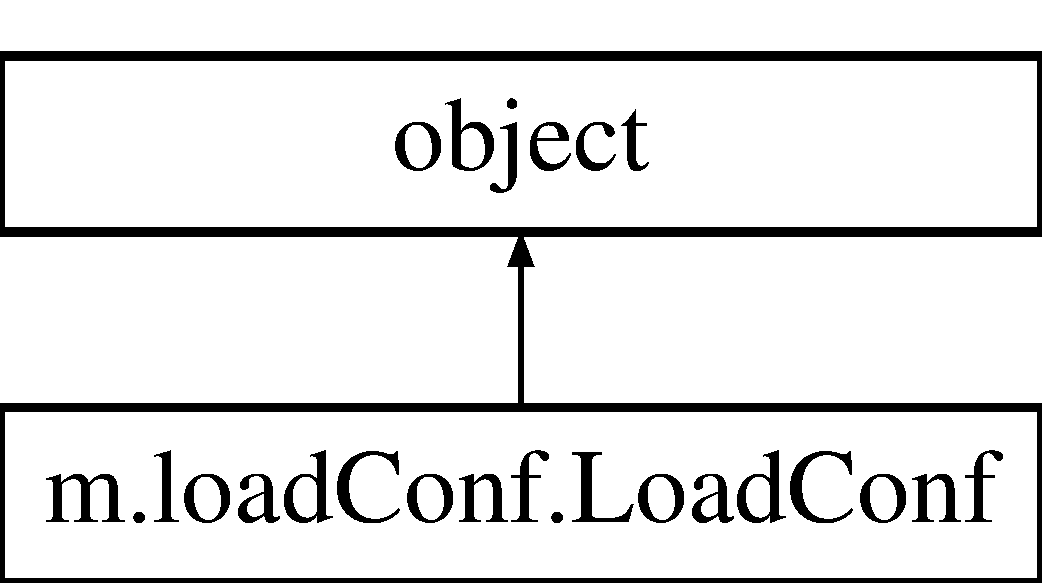
\includegraphics[height=2.000000cm]{classm_1_1load_conf_1_1_load_conf}
\end{center}
\end{figure}
\subsection*{Public Member Functions}
\begin{DoxyCompactItemize}
\item 
def \hyperlink{classm_1_1load_conf_1_1_load_conf_ae831fd20f8770ee87d26e6c34febea5b}{load\-Value}
\item 
def \hyperlink{classm_1_1load_conf_1_1_load_conf_ac3be38f004ccea7185b261b0e16ccbc2}{is\-Blind}
\item 
\hypertarget{classm_1_1load_conf_1_1_load_conf_a90af7dd2fda7be0dea8b4a65ce38eb2f}{def {\bfseries ip\-Camera}}\label{classm_1_1load_conf_1_1_load_conf_a90af7dd2fda7be0dea8b4a65ce38eb2f}

\item 
\hypertarget{classm_1_1load_conf_1_1_load_conf_a6db2941a05e53d8eb028c38dce89a5dc}{def {\bfseries port\-Camera}}\label{classm_1_1load_conf_1_1_load_conf_a6db2941a05e53d8eb028c38dce89a5dc}

\item 
\hypertarget{classm_1_1load_conf_1_1_load_conf_a855f4f41860aa066b816236cc074f471}{def {\bfseries ip\-Serv}}\label{classm_1_1load_conf_1_1_load_conf_a855f4f41860aa066b816236cc074f471}

\item 
\hypertarget{classm_1_1load_conf_1_1_load_conf_a5318b43bf50966159fee6a88bce49e45}{def {\bfseries port\-Serv}}\label{classm_1_1load_conf_1_1_load_conf_a5318b43bf50966159fee6a88bce49e45}

\end{DoxyCompactItemize}


\subsection{Detailed Description}
\begin{DoxyVerb}Loading configuration file\end{DoxyVerb}
 

\subsection{Member Function Documentation}
\hypertarget{classm_1_1load_conf_1_1_load_conf_ac3be38f004ccea7185b261b0e16ccbc2}{\index{m\-::load\-Conf\-::\-Load\-Conf@{m\-::load\-Conf\-::\-Load\-Conf}!is\-Blind@{is\-Blind}}
\index{is\-Blind@{is\-Blind}!m::loadConf::LoadConf@{m\-::load\-Conf\-::\-Load\-Conf}}
\subsubsection[{is\-Blind}]{\setlength{\rightskip}{0pt plus 5cm}def m.\-load\-Conf.\-Load\-Conf.\-is\-Blind (
\begin{DoxyParamCaption}
\item[{}]{self}
\end{DoxyParamCaption}
)}}\label{classm_1_1load_conf_1_1_load_conf_ac3be38f004ccea7185b261b0e16ccbc2}
\begin{DoxyVerb}Return true if configuration is for Blind
Else false
\end{DoxyVerb}
 \hypertarget{classm_1_1load_conf_1_1_load_conf_ae831fd20f8770ee87d26e6c34febea5b}{\index{m\-::load\-Conf\-::\-Load\-Conf@{m\-::load\-Conf\-::\-Load\-Conf}!load\-Value@{load\-Value}}
\index{load\-Value@{load\-Value}!m::loadConf::LoadConf@{m\-::load\-Conf\-::\-Load\-Conf}}
\subsubsection[{load\-Value}]{\setlength{\rightskip}{0pt plus 5cm}def m.\-load\-Conf.\-Load\-Conf.\-load\-Value (
\begin{DoxyParamCaption}
\item[{}]{self, }
\item[{}]{key}
\end{DoxyParamCaption}
)}}\label{classm_1_1load_conf_1_1_load_conf_ae831fd20f8770ee87d26e6c34febea5b}
\begin{DoxyVerb}Return the value associate to the key into conf file (fichier/conf)
Else return "error"
\end{DoxyVerb}
 

The documentation for this class was generated from the following file\-:\begin{DoxyCompactItemize}
\item 
m/load\-Conf.\-py\end{DoxyCompactItemize}

\hypertarget{classm_1_1log_1_1_log}{\section{m.\-log.\-Log Class Reference}
\label{classm_1_1log_1_1_log}\index{m.\-log.\-Log@{m.\-log.\-Log}}
}
Inheritance diagram for m.\-log.\-Log\-:\begin{figure}[H]
\begin{center}
\leavevmode
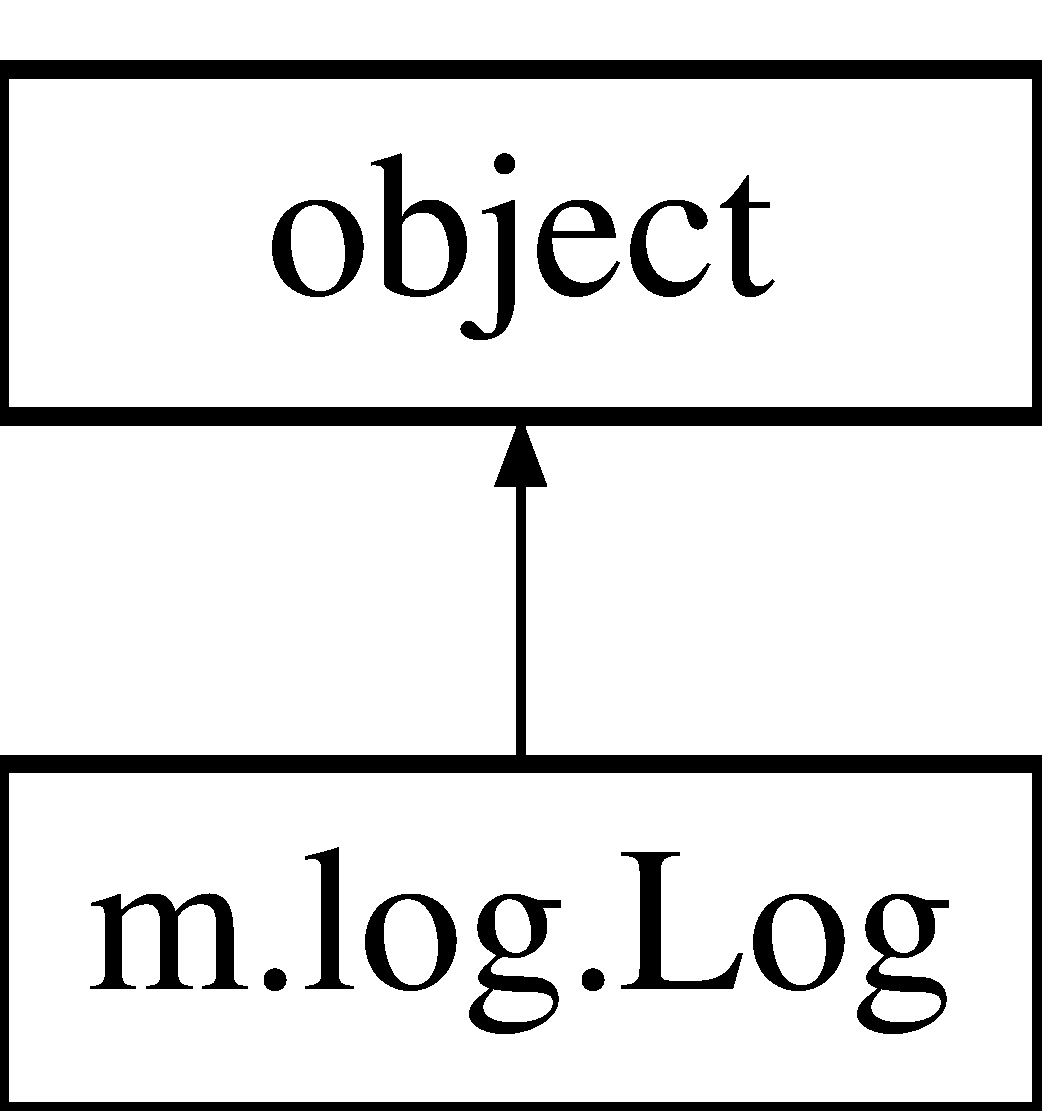
\includegraphics[height=2.000000cm]{classm_1_1log_1_1_log}
\end{center}
\end{figure}
\subsection*{Public Member Functions}
\begin{DoxyCompactItemize}
\item 
def \hyperlink{classm_1_1log_1_1_log_a427aee1729c3bfbc0683753f2f5a5e8b}{\-\_\-\-\_\-init\-\_\-\-\_\-}
\item 
def \hyperlink{classm_1_1log_1_1_log_ae0287ddb37e9c5e3ac794a8ff7bbbe14}{print\-L}
\end{DoxyCompactItemize}
\subsection*{Public Attributes}
\begin{DoxyCompactItemize}
\item 
\hypertarget{classm_1_1log_1_1_log_a5459d297a6dbbd80ffd63adad30c6d9a}{{\bfseries logger}}\label{classm_1_1log_1_1_log_a5459d297a6dbbd80ffd63adad30c6d9a}

\end{DoxyCompactItemize}


\subsection{Detailed Description}
\begin{DoxyVerb}Log Manager
\end{DoxyVerb}
 

\subsection{Constructor \& Destructor Documentation}
\hypertarget{classm_1_1log_1_1_log_a427aee1729c3bfbc0683753f2f5a5e8b}{\index{m\-::log\-::\-Log@{m\-::log\-::\-Log}!\-\_\-\-\_\-init\-\_\-\-\_\-@{\-\_\-\-\_\-init\-\_\-\-\_\-}}
\index{\-\_\-\-\_\-init\-\_\-\-\_\-@{\-\_\-\-\_\-init\-\_\-\-\_\-}!m::log::Log@{m\-::log\-::\-Log}}
\subsubsection[{\-\_\-\-\_\-init\-\_\-\-\_\-}]{\setlength{\rightskip}{0pt plus 5cm}def m.\-log.\-Log.\-\_\-\-\_\-init\-\_\-\-\_\- (
\begin{DoxyParamCaption}
\item[{}]{self}
\end{DoxyParamCaption}
)}}\label{classm_1_1log_1_1_log_a427aee1729c3bfbc0683753f2f5a5e8b}
\begin{DoxyVerb}Define 3 differents log :
activity.log -> all activity server
warning.log -> only warning server (including illegal acess)
error.log' -> error server
Write all message on terminal too
\end{DoxyVerb}
 

\subsection{Member Function Documentation}
\hypertarget{classm_1_1log_1_1_log_ae0287ddb37e9c5e3ac794a8ff7bbbe14}{\index{m\-::log\-::\-Log@{m\-::log\-::\-Log}!print\-L@{print\-L}}
\index{print\-L@{print\-L}!m::log::Log@{m\-::log\-::\-Log}}
\subsubsection[{print\-L}]{\setlength{\rightskip}{0pt plus 5cm}def m.\-log.\-Log.\-print\-L (
\begin{DoxyParamCaption}
\item[{}]{self, }
\item[{}]{p\-Msg, }
\item[{}]{p\-Lvl}
\end{DoxyParamCaption}
)}}\label{classm_1_1log_1_1_log_ae0287ddb37e9c5e3ac794a8ff7bbbe14}
\begin{DoxyVerb}Add color and write in log with an define level
pMsg : message to write in log
pLvl : level of log message
\end{DoxyVerb}
 

The documentation for this class was generated from the following file\-:\begin{DoxyCompactItemize}
\item 
m/log.\-py\end{DoxyCompactItemize}

\hypertarget{classm_1_1login_1_1_login}{\section{m.\-login.\-Login Class Reference}
\label{classm_1_1login_1_1_login}\index{m.\-login.\-Login@{m.\-login.\-Login}}
}
Inheritance diagram for m.\-login.\-Login\-:\begin{figure}[H]
\begin{center}
\leavevmode
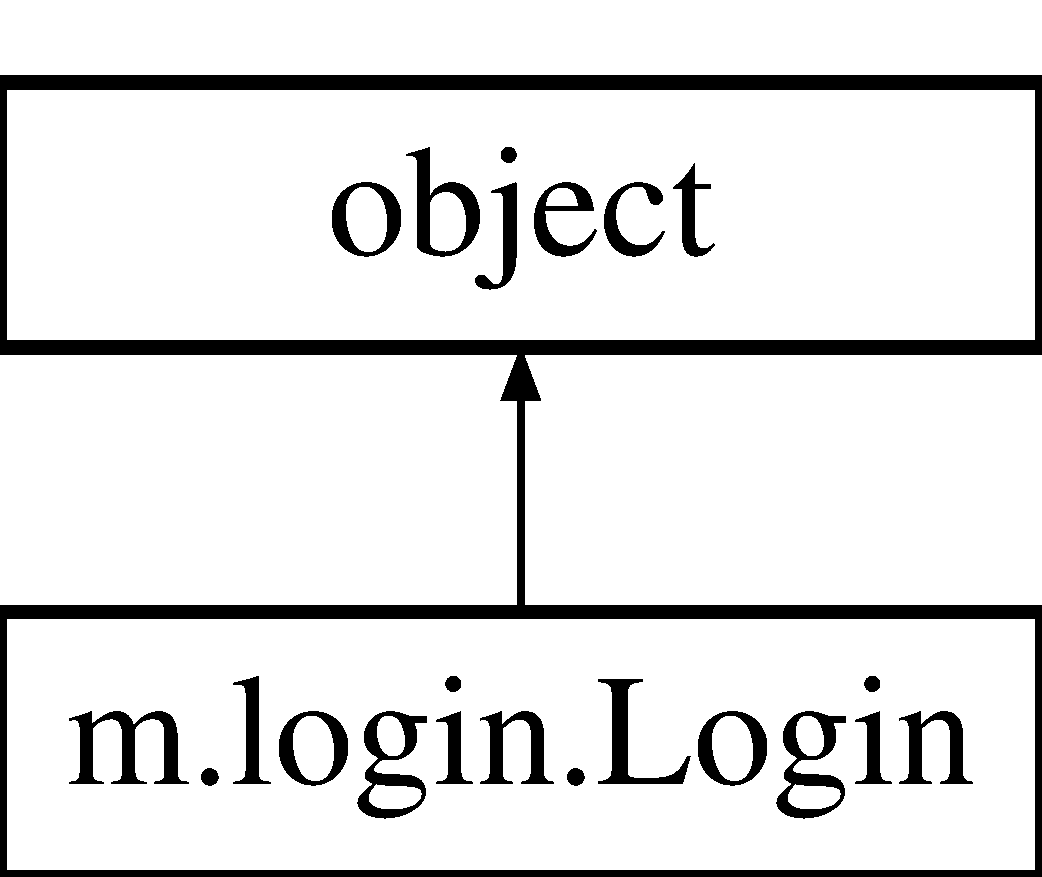
\includegraphics[height=2.000000cm]{classm_1_1login_1_1_login}
\end{center}
\end{figure}
\subsection*{Public Member Functions}
\begin{DoxyCompactItemize}
\item 
def \hyperlink{classm_1_1login_1_1_login_ab5b1758239ba271d5e8ce570a1f99f44}{check\-Login}
\end{DoxyCompactItemize}


\subsection{Detailed Description}
\begin{DoxyVerb}Login manager
\end{DoxyVerb}
 

\subsection{Member Function Documentation}
\hypertarget{classm_1_1login_1_1_login_ab5b1758239ba271d5e8ce570a1f99f44}{\index{m\-::login\-::\-Login@{m\-::login\-::\-Login}!check\-Login@{check\-Login}}
\index{check\-Login@{check\-Login}!m::login::Login@{m\-::login\-::\-Login}}
\subsubsection[{check\-Login}]{\setlength{\rightskip}{0pt plus 5cm}def m.\-login.\-Login.\-check\-Login (
\begin{DoxyParamCaption}
\item[{}]{self, }
\item[{}]{p\-Log, }
\item[{}]{p\-Passwd}
\end{DoxyParamCaption}
)}}\label{classm_1_1login_1_1_login_ab5b1758239ba271d5e8ce570a1f99f44}
\begin{DoxyVerb}Check if login and password are correct (in file fichier/allow)
password in File are hash (sha224)
pLog : id login
pPasswd : password
return : true if correct login
false else
\end{DoxyVerb}
 

The documentation for this class was generated from the following file\-:\begin{DoxyCompactItemize}
\item 
m/login.\-py\end{DoxyCompactItemize}

\hypertarget{classm_1_1log_1_1lvl}{\section{m.\-log.\-lvl Class Reference}
\label{classm_1_1log_1_1lvl}\index{m.\-log.\-lvl@{m.\-log.\-lvl}}
}
\subsection*{Static Public Attributes}
\begin{DoxyCompactItemize}
\item 
\hypertarget{classm_1_1log_1_1lvl_a02a7ab0eae805ef6299d02724d23a1e9}{int {\bfseries N\-O\-T\-S\-E\-T} = 0}\label{classm_1_1log_1_1lvl_a02a7ab0eae805ef6299d02724d23a1e9}

\item 
\hypertarget{classm_1_1log_1_1lvl_ae27313c8845fa44688f16b1e7e9a90db}{int {\bfseries D\-E\-B\-U\-G} = 10}\label{classm_1_1log_1_1lvl_ae27313c8845fa44688f16b1e7e9a90db}

\item 
\hypertarget{classm_1_1log_1_1lvl_abbbf01d307d70a0769983ff3a2576fdf}{int {\bfseries I\-N\-F\-O} = 20}\label{classm_1_1log_1_1lvl_abbbf01d307d70a0769983ff3a2576fdf}

\item 
\hypertarget{classm_1_1log_1_1lvl_a5b4f6d8f38839f94dd2de426f0086534}{int {\bfseries S\-U\-C\-C\-E\-S\-S} = 25}\label{classm_1_1log_1_1lvl_a5b4f6d8f38839f94dd2de426f0086534}

\item 
\hypertarget{classm_1_1log_1_1lvl_a444610aad5eee02a7219ca36f6855058}{int {\bfseries W\-A\-R\-N\-I\-N\-G} = 30}\label{classm_1_1log_1_1lvl_a444610aad5eee02a7219ca36f6855058}

\item 
\hypertarget{classm_1_1log_1_1lvl_a6cb43432a2d85baa77100764582e3348}{int {\bfseries F\-A\-I\-L} = 40}\label{classm_1_1log_1_1lvl_a6cb43432a2d85baa77100764582e3348}

\end{DoxyCompactItemize}


\subsection{Detailed Description}
\begin{DoxyVerb}Define constant value for level log
\end{DoxyVerb}
 

The documentation for this class was generated from the following file\-:\begin{DoxyCompactItemize}
\item 
m/log.\-py\end{DoxyCompactItemize}

\hypertarget{classsuper_tornado_1_1_main_handler}{\section{super\-Tornado.\-Main\-Handler Class Reference}
\label{classsuper_tornado_1_1_main_handler}\index{super\-Tornado.\-Main\-Handler@{super\-Tornado.\-Main\-Handler}}
}
Inheritance diagram for super\-Tornado.\-Main\-Handler\-:\begin{figure}[H]
\begin{center}
\leavevmode
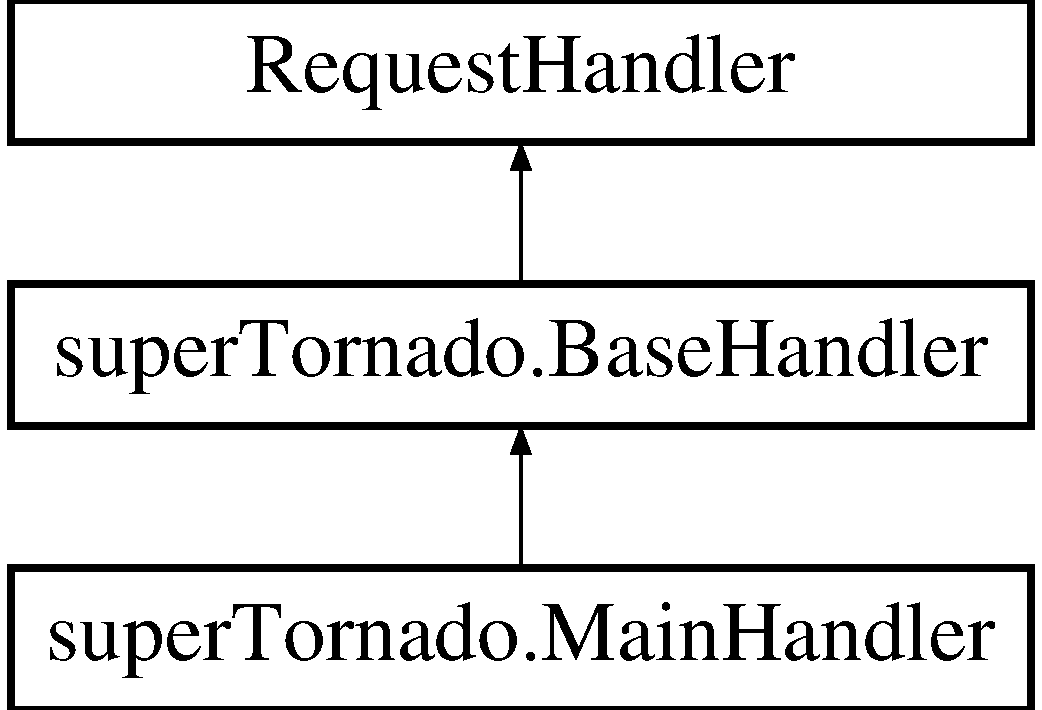
\includegraphics[height=3.000000cm]{classsuper_tornado_1_1_main_handler}
\end{center}
\end{figure}
\subsection*{Public Member Functions}
\begin{DoxyCompactItemize}
\item 
def \hyperlink{classsuper_tornado_1_1_main_handler_aa07ddde9b0a5bd006a055858ffef03cd}{get}
\item 
def \hyperlink{classsuper_tornado_1_1_main_handler_a34b9f9761f25b951e452954252e82deb}{post}
\end{DoxyCompactItemize}


\subsection{Detailed Description}
\begin{DoxyVerb}Main web page : / in http sever
\end{DoxyVerb}
 

\subsection{Member Function Documentation}
\hypertarget{classsuper_tornado_1_1_main_handler_aa07ddde9b0a5bd006a055858ffef03cd}{\index{super\-Tornado\-::\-Main\-Handler@{super\-Tornado\-::\-Main\-Handler}!get@{get}}
\index{get@{get}!superTornado::MainHandler@{super\-Tornado\-::\-Main\-Handler}}
\subsubsection[{get}]{\setlength{\rightskip}{0pt plus 5cm}def super\-Tornado.\-Main\-Handler.\-get (
\begin{DoxyParamCaption}
\item[{}]{self}
\end{DoxyParamCaption}
)}}\label{classsuper_tornado_1_1_main_handler_aa07ddde9b0a5bd006a055858ffef03cd}
\begin{DoxyVerb}GET request -> return index.html where user can login
\end{DoxyVerb}
 \hypertarget{classsuper_tornado_1_1_main_handler_a34b9f9761f25b951e452954252e82deb}{\index{super\-Tornado\-::\-Main\-Handler@{super\-Tornado\-::\-Main\-Handler}!post@{post}}
\index{post@{post}!superTornado::MainHandler@{super\-Tornado\-::\-Main\-Handler}}
\subsubsection[{post}]{\setlength{\rightskip}{0pt plus 5cm}def super\-Tornado.\-Main\-Handler.\-post (
\begin{DoxyParamCaption}
\item[{}]{self}
\end{DoxyParamCaption}
)}}\label{classsuper_tornado_1_1_main_handler_a34b9f9761f25b951e452954252e82deb}
\begin{DoxyVerb}POST request -> try to connect user with parameter POST (iden and paswd)
if connection sucessfull
    go to the /video page (VideoHandler)
else
    go to the /unauthorized page (UnauthorizedHandler)
\end{DoxyVerb}
 

The documentation for this class was generated from the following file\-:\begin{DoxyCompactItemize}
\item 
super\-Tornado.\-py\end{DoxyCompactItemize}

\hypertarget{classm_1_1log_1_1_single_level_filter}{\section{m.\-log.\-Single\-Level\-Filter Class Reference}
\label{classm_1_1log_1_1_single_level_filter}\index{m.\-log.\-Single\-Level\-Filter@{m.\-log.\-Single\-Level\-Filter}}
}
Inheritance diagram for m.\-log.\-Single\-Level\-Filter\-:\begin{figure}[H]
\begin{center}
\leavevmode
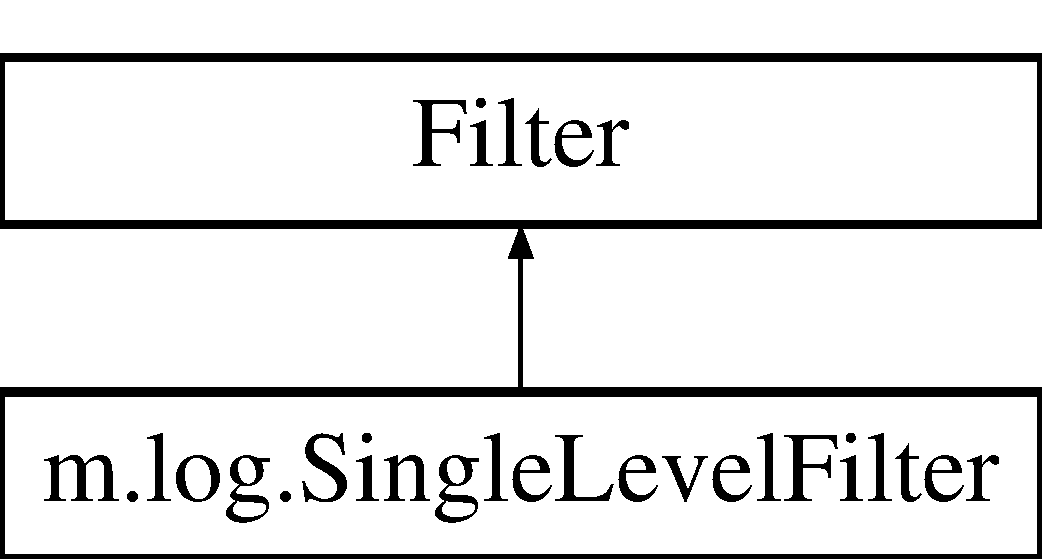
\includegraphics[height=2.000000cm]{classm_1_1log_1_1_single_level_filter}
\end{center}
\end{figure}
\subsection*{Public Member Functions}
\begin{DoxyCompactItemize}
\item 
def \hyperlink{classm_1_1log_1_1_single_level_filter_a0d9e04941fa9c8c37e6d49a2a38cc7e0}{\-\_\-\-\_\-init\-\_\-\-\_\-}
\end{DoxyCompactItemize}
\subsection*{Public Attributes}
\begin{DoxyCompactItemize}
\item 
\hypertarget{classm_1_1log_1_1_single_level_filter_ace7b691dfece2684f31ef1843cee6120}{{\bfseries passlevel}}\label{classm_1_1log_1_1_single_level_filter_ace7b691dfece2684f31ef1843cee6120}

\item 
\hypertarget{classm_1_1log_1_1_single_level_filter_a0d2c89b31ff79eff990febd51be3c127}{{\bfseries reject}}\label{classm_1_1log_1_1_single_level_filter_a0d2c89b31ff79eff990febd51be3c127}

\end{DoxyCompactItemize}


\subsection{Detailed Description}
\begin{DoxyVerb}Filter for one level\end{DoxyVerb}
 

\subsection{Constructor \& Destructor Documentation}
\hypertarget{classm_1_1log_1_1_single_level_filter_a0d9e04941fa9c8c37e6d49a2a38cc7e0}{\index{m\-::log\-::\-Single\-Level\-Filter@{m\-::log\-::\-Single\-Level\-Filter}!\-\_\-\-\_\-init\-\_\-\-\_\-@{\-\_\-\-\_\-init\-\_\-\-\_\-}}
\index{\-\_\-\-\_\-init\-\_\-\-\_\-@{\-\_\-\-\_\-init\-\_\-\-\_\-}!m::log::SingleLevelFilter@{m\-::log\-::\-Single\-Level\-Filter}}
\subsubsection[{\-\_\-\-\_\-init\-\_\-\-\_\-}]{\setlength{\rightskip}{0pt plus 5cm}def m.\-log.\-Single\-Level\-Filter.\-\_\-\-\_\-init\-\_\-\-\_\- (
\begin{DoxyParamCaption}
\item[{}]{self, }
\item[{}]{passlevel, }
\item[{}]{reject}
\end{DoxyParamCaption}
)}}\label{classm_1_1log_1_1_single_level_filter_a0d9e04941fa9c8c37e6d49a2a38cc7e0}
\begin{DoxyVerb}Constructor
passlevel : level to filter
reject : true on reject state
\end{DoxyVerb}
 

The documentation for this class was generated from the following file\-:\begin{DoxyCompactItemize}
\item 
m/log.\-py\end{DoxyCompactItemize}

\hypertarget{classsuper_tornado_1_1_unauthorized_handler}{\section{super\-Tornado.\-Unauthorized\-Handler Class Reference}
\label{classsuper_tornado_1_1_unauthorized_handler}\index{super\-Tornado.\-Unauthorized\-Handler@{super\-Tornado.\-Unauthorized\-Handler}}
}
Inheritance diagram for super\-Tornado.\-Unauthorized\-Handler\-:\begin{figure}[H]
\begin{center}
\leavevmode
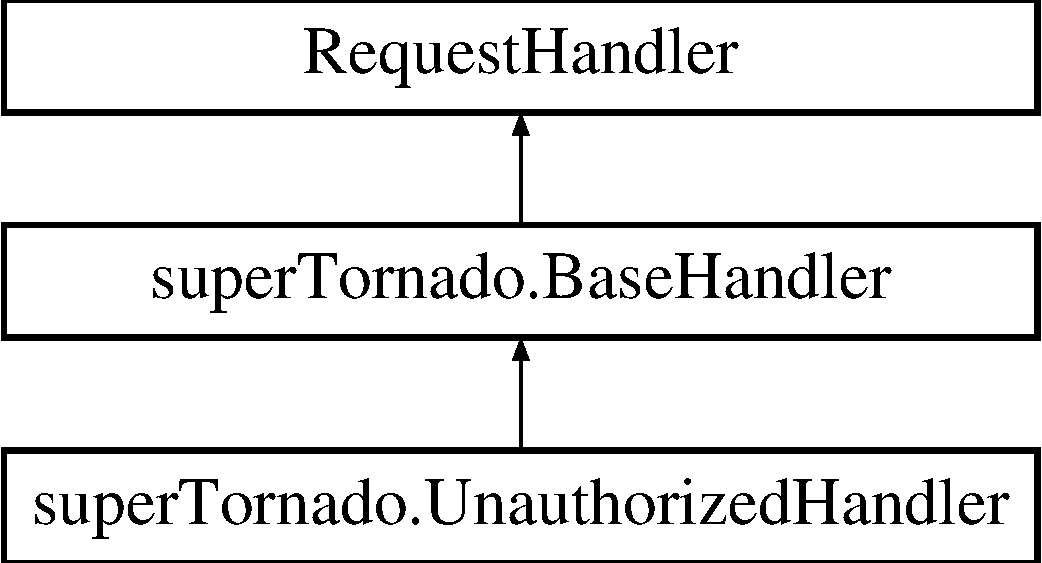
\includegraphics[height=3.000000cm]{classsuper_tornado_1_1_unauthorized_handler}
\end{center}
\end{figure}
\subsection*{Public Member Functions}
\begin{DoxyCompactItemize}
\item 
def \hyperlink{classsuper_tornado_1_1_unauthorized_handler_abd4e0e51dd5bae66506808c6e2beeb8d}{get}
\item 
def \hyperlink{classsuper_tornado_1_1_unauthorized_handler_af4b77e66e008a11b82cad37160e4c5d9}{post}
\end{DoxyCompactItemize}


\subsection{Detailed Description}
\begin{DoxyVerb}Unauthorized web page : /unauthorized in http server
\end{DoxyVerb}
 

\subsection{Member Function Documentation}
\hypertarget{classsuper_tornado_1_1_unauthorized_handler_abd4e0e51dd5bae66506808c6e2beeb8d}{\index{super\-Tornado\-::\-Unauthorized\-Handler@{super\-Tornado\-::\-Unauthorized\-Handler}!get@{get}}
\index{get@{get}!superTornado::UnauthorizedHandler@{super\-Tornado\-::\-Unauthorized\-Handler}}
\subsubsection[{get}]{\setlength{\rightskip}{0pt plus 5cm}def super\-Tornado.\-Unauthorized\-Handler.\-get (
\begin{DoxyParamCaption}
\item[{}]{self}
\end{DoxyParamCaption}
)}}\label{classsuper_tornado_1_1_unauthorized_handler_abd4e0e51dd5bae66506808c6e2beeb8d}
\begin{DoxyVerb}GET request -> show the illegal.html page
\end{DoxyVerb}
 \hypertarget{classsuper_tornado_1_1_unauthorized_handler_af4b77e66e008a11b82cad37160e4c5d9}{\index{super\-Tornado\-::\-Unauthorized\-Handler@{super\-Tornado\-::\-Unauthorized\-Handler}!post@{post}}
\index{post@{post}!superTornado::UnauthorizedHandler@{super\-Tornado\-::\-Unauthorized\-Handler}}
\subsubsection[{post}]{\setlength{\rightskip}{0pt plus 5cm}def super\-Tornado.\-Unauthorized\-Handler.\-post (
\begin{DoxyParamCaption}
\item[{}]{self}
\end{DoxyParamCaption}
)}}\label{classsuper_tornado_1_1_unauthorized_handler_af4b77e66e008a11b82cad37160e4c5d9}
\begin{DoxyVerb}POST request ->
if parameter POST force == 1
    force acess to camera
else
     go to / page (MainHandler)
\end{DoxyVerb}
 

The documentation for this class was generated from the following file\-:\begin{DoxyCompactItemize}
\item 
c/super\-Tornado.\-py\end{DoxyCompactItemize}

\hypertarget{classsuper_tornado_1_1_video_handler}{\section{super\-Tornado.\-Video\-Handler Class Reference}
\label{classsuper_tornado_1_1_video_handler}\index{super\-Tornado.\-Video\-Handler@{super\-Tornado.\-Video\-Handler}}
}
Inheritance diagram for super\-Tornado.\-Video\-Handler\-:\begin{figure}[H]
\begin{center}
\leavevmode
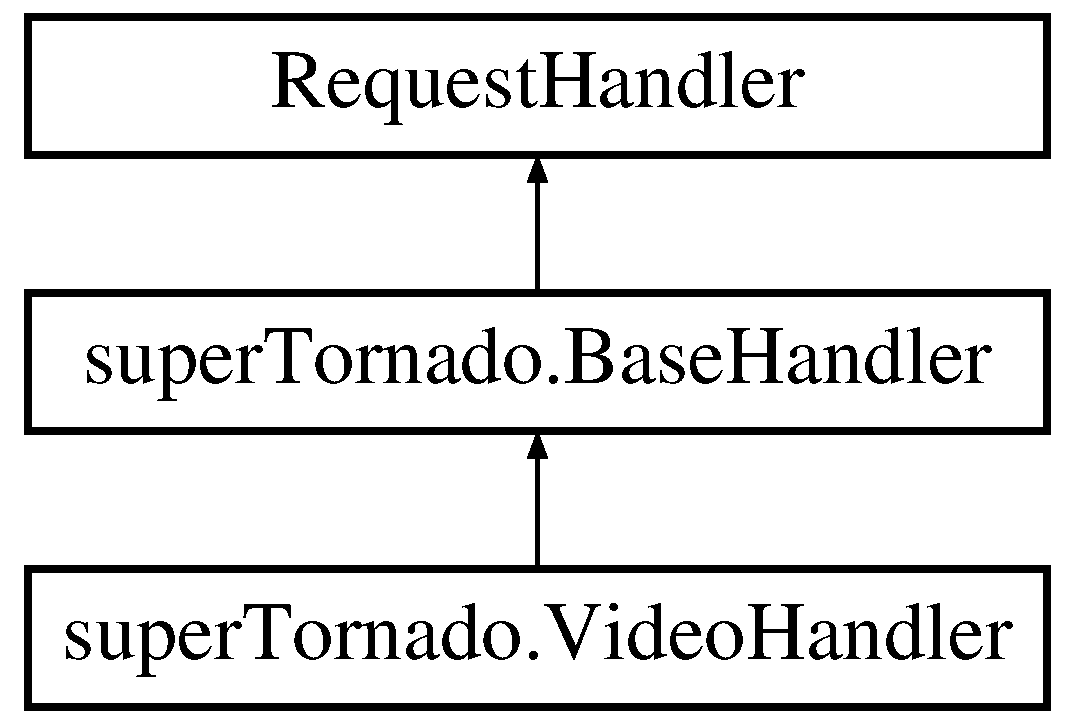
\includegraphics[height=3.000000cm]{classsuper_tornado_1_1_video_handler}
\end{center}
\end{figure}
\subsection*{Public Member Functions}
\begin{DoxyCompactItemize}
\item 
def \hyperlink{classsuper_tornado_1_1_video_handler_a349cb4813821fec69a5ae01ab1067b53}{get}
\end{DoxyCompactItemize}


\subsection{Detailed Description}
\begin{DoxyVerb}Video web page : /video in http sever
\end{DoxyVerb}
 

\subsection{Member Function Documentation}
\hypertarget{classsuper_tornado_1_1_video_handler_a349cb4813821fec69a5ae01ab1067b53}{\index{super\-Tornado\-::\-Video\-Handler@{super\-Tornado\-::\-Video\-Handler}!get@{get}}
\index{get@{get}!superTornado::VideoHandler@{super\-Tornado\-::\-Video\-Handler}}
\subsubsection[{get}]{\setlength{\rightskip}{0pt plus 5cm}def super\-Tornado.\-Video\-Handler.\-get (
\begin{DoxyParamCaption}
\item[{}]{self}
\end{DoxyParamCaption}
)}}\label{classsuper_tornado_1_1_video_handler_a349cb4813821fec69a5ae01ab1067b53}
\begin{DoxyVerb}GET request ->
If user is connected return video.html who
    allow with websocket (WSocketHandler) to see the video of the camera
Else
    go to main page (MainHandler)
\end{DoxyVerb}
 

The documentation for this class was generated from the following file\-:\begin{DoxyCompactItemize}
\item 
c/super\-Tornado.\-py\end{DoxyCompactItemize}

\hypertarget{classsuper_tornado_1_1_w_socket_handler}{\section{super\-Tornado.\-W\-Socket\-Handler Class Reference}
\label{classsuper_tornado_1_1_w_socket_handler}\index{super\-Tornado.\-W\-Socket\-Handler@{super\-Tornado.\-W\-Socket\-Handler}}
}
Inheritance diagram for super\-Tornado.\-W\-Socket\-Handler\-:\begin{figure}[H]
\begin{center}
\leavevmode
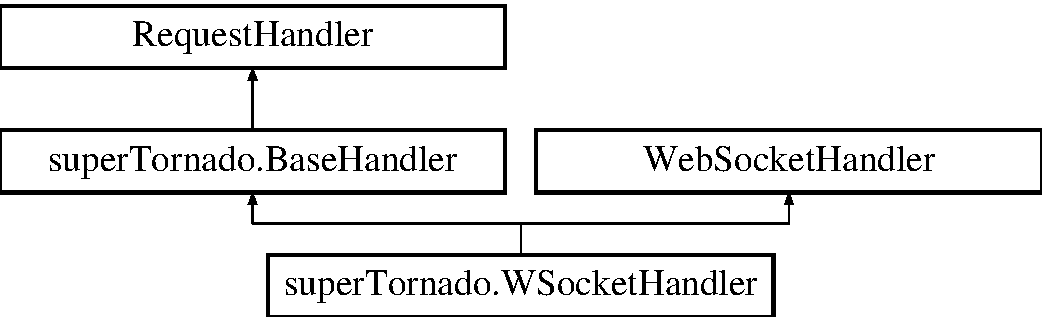
\includegraphics[height=3.000000cm]{classsuper_tornado_1_1_w_socket_handler}
\end{center}
\end{figure}
\subsection*{Public Member Functions}
\begin{DoxyCompactItemize}
\item 
def \hyperlink{classsuper_tornado_1_1_w_socket_handler_a93c6a7682da1900113bf2f0894b93fa2}{open}
\item 
def \hyperlink{classsuper_tornado_1_1_w_socket_handler_a4ef2fe7a6016b72f7d80c80260f2ceae}{on\-\_\-message}
\item 
def \hyperlink{classsuper_tornado_1_1_w_socket_handler_acd974cfb26b4f7461cb631407a7e3c1d}{on\-\_\-close}
\item 
def \hyperlink{classsuper_tornado_1_1_w_socket_handler_ae0ed9d69a6bb69cc74a394c8973fbbb8}{send\-\_\-signal\-\_\-house}
\item 
def \hyperlink{classsuper_tornado_1_1_w_socket_handler_a9a80cbbe4a4a87dd7eca485ec6b9e04b}{send\-\_\-image}
\end{DoxyCompactItemize}


\subsection{Detailed Description}
\begin{DoxyVerb}/socket in http server
websocket definition
\end{DoxyVerb}
 

\subsection{Member Function Documentation}
\hypertarget{classsuper_tornado_1_1_w_socket_handler_acd974cfb26b4f7461cb631407a7e3c1d}{\index{super\-Tornado\-::\-W\-Socket\-Handler@{super\-Tornado\-::\-W\-Socket\-Handler}!on\-\_\-close@{on\-\_\-close}}
\index{on\-\_\-close@{on\-\_\-close}!superTornado::WSocketHandler@{super\-Tornado\-::\-W\-Socket\-Handler}}
\subsubsection[{on\-\_\-close}]{\setlength{\rightskip}{0pt plus 5cm}def super\-Tornado.\-W\-Socket\-Handler.\-on\-\_\-close (
\begin{DoxyParamCaption}
\item[{}]{self}
\end{DoxyParamCaption}
)}}\label{classsuper_tornado_1_1_w_socket_handler_acd974cfb26b4f7461cb631407a7e3c1d}
\begin{DoxyVerb}Socket connection Connection
Alert unhabitant with the good signal
\end{DoxyVerb}
 \hypertarget{classsuper_tornado_1_1_w_socket_handler_a4ef2fe7a6016b72f7d80c80260f2ceae}{\index{super\-Tornado\-::\-W\-Socket\-Handler@{super\-Tornado\-::\-W\-Socket\-Handler}!on\-\_\-message@{on\-\_\-message}}
\index{on\-\_\-message@{on\-\_\-message}!superTornado::WSocketHandler@{super\-Tornado\-::\-W\-Socket\-Handler}}
\subsubsection[{on\-\_\-message}]{\setlength{\rightskip}{0pt plus 5cm}def super\-Tornado.\-W\-Socket\-Handler.\-on\-\_\-message (
\begin{DoxyParamCaption}
\item[{}]{self, }
\item[{}]{msg}
\end{DoxyParamCaption}
)}}\label{classsuper_tornado_1_1_w_socket_handler_a4ef2fe7a6016b72f7d80c80260f2ceae}
\begin{DoxyVerb}Client Ask For Image
\end{DoxyVerb}
 \hypertarget{classsuper_tornado_1_1_w_socket_handler_a93c6a7682da1900113bf2f0894b93fa2}{\index{super\-Tornado\-::\-W\-Socket\-Handler@{super\-Tornado\-::\-W\-Socket\-Handler}!open@{open}}
\index{open@{open}!superTornado::WSocketHandler@{super\-Tornado\-::\-W\-Socket\-Handler}}
\subsubsection[{open}]{\setlength{\rightskip}{0pt plus 5cm}def super\-Tornado.\-W\-Socket\-Handler.\-open (
\begin{DoxyParamCaption}
\item[{}]{self}
\end{DoxyParamCaption}
)}}\label{classsuper_tornado_1_1_w_socket_handler_a93c6a7682da1900113bf2f0894b93fa2}
\begin{DoxyVerb}Open socket request ->
if is a connect user
    open connection socket, alert the unhabitant with the good signal
else
    don't open connection
\end{DoxyVerb}
 \hypertarget{classsuper_tornado_1_1_w_socket_handler_a9a80cbbe4a4a87dd7eca485ec6b9e04b}{\index{super\-Tornado\-::\-W\-Socket\-Handler@{super\-Tornado\-::\-W\-Socket\-Handler}!send\-\_\-image@{send\-\_\-image}}
\index{send\-\_\-image@{send\-\_\-image}!superTornado::WSocketHandler@{super\-Tornado\-::\-W\-Socket\-Handler}}
\subsubsection[{send\-\_\-image}]{\setlength{\rightskip}{0pt plus 5cm}def super\-Tornado.\-W\-Socket\-Handler.\-send\-\_\-image (
\begin{DoxyParamCaption}
\item[{}]{self}
\end{DoxyParamCaption}
)}}\label{classsuper_tornado_1_1_w_socket_handler_a9a80cbbe4a4a87dd7eca485ec6b9e04b}
\begin{DoxyVerb}Allow send the image in the websocket
\end{DoxyVerb}
 \hypertarget{classsuper_tornado_1_1_w_socket_handler_ae0ed9d69a6bb69cc74a394c8973fbbb8}{\index{super\-Tornado\-::\-W\-Socket\-Handler@{super\-Tornado\-::\-W\-Socket\-Handler}!send\-\_\-signal\-\_\-house@{send\-\_\-signal\-\_\-house}}
\index{send\-\_\-signal\-\_\-house@{send\-\_\-signal\-\_\-house}!superTornado::WSocketHandler@{super\-Tornado\-::\-W\-Socket\-Handler}}
\subsubsection[{send\-\_\-signal\-\_\-house}]{\setlength{\rightskip}{0pt plus 5cm}def super\-Tornado.\-W\-Socket\-Handler.\-send\-\_\-signal\-\_\-house (
\begin{DoxyParamCaption}
\item[{}]{self, }
\item[{}]{p\-Rq}
\end{DoxyParamCaption}
)}}\label{classsuper_tornado_1_1_w_socket_handler_ae0ed9d69a6bb69cc74a394c8973fbbb8}
\begin{DoxyVerb}Allow send pRq request to the house
\end{DoxyVerb}
 

The documentation for this class was generated from the following file\-:\begin{DoxyCompactItemize}
\item 
super\-Tornado.\-py\end{DoxyCompactItemize}

%--- End generated contents ---

% Index
\newpage
\phantomsection
\addcontentsline{toc}{chapter}{Index}
\printindex

\end{document}
